\documentclass{article}
\usepackage{cmap}
\usepackage[utf8]{inputenc}
\usepackage[english,ukrainian]{babel}
\usepackage{graphicx}
\usepackage{geometry}
\usepackage{listings}
\usepackage{float}
\geometry{
	a4paper,
	left=20mm,
	right=20mm,
	top=20mm,
	bottom=20mm
}
\lstset{
	language=c,
	tabsize=4,
	keepspaces,
	showstringspaces=false,
}
\graphicspath{ {./pictures} }
\setlength{\parindent}{4em}

\newcommand\subject{Алгоритми та структури даних}
\newcommand\lecturer{доцент кафедри ПЗ\\Коротєєва Т.О.}
\newcommand\teacher{асистент кафедри ПЗ\\Франко А.В.}
\newcommand\mygroup{ПЗ-22}
\newcommand\lab{4}
\newcommand\theme{Метод швидкого сортування}
\newcommand\purpose{Вивчити алгоритм швидкого сортування. Здійснити програмну реалізацію алгоритму швидкого сортування. Дослідити швидкодію алгоритму швидкого сортування}

\begin{document}
	\begin{normalsize}
		\begin{titlepage}
			\thispagestyle{empty}
			\begin{center}
				\textbf{МІНІСТЕРСТВО ОСВІТИ І НАУКИ УКРАЇНИ\\
					НАЦІОНАЛЬНИЙ УНІВЕРСИТЕТ "ЛЬВІВСЬКА ПОЛІТЕХНІКА"}
			\end{center}
			\begin{flushright}
				Інститут \textbf{КНІТ}\\
				Кафедра \textbf{ПЗ}
			\end{flushright}
			\vspace{200pt}
			\begin{center}
				\textbf{ЗВІТ}\\
				\vspace{10pt}
				До лабораторної роботи № \lab\\
				\textbf{На тему}: “\textit{\theme}”\\
				\textbf{З дисципліни}: “\subject”
			\end{center}
			\vspace{112pt}
			\begin{flushright}
				
				\textbf{Лектор}:\\
				\lecturer\\
				\vspace{28pt}
				\textbf{Виконав}:\\
				
				студент групи \mygroup\\
				Коваленко Д.М.\\
				\vspace{28pt}
				\textbf{Прийняв}:\\
				
				\teacher\\
				
				\vspace{28pt}
				«\rule{1cm}{0.15mm}» \rule{1.5cm}{0.15mm} 2022 р.\\
				$\sum$ = \rule{1cm}{0.15mm}……………\\
				
			\end{flushright}
			\vspace{\fill}
			\begin{center}
				\textbf{Львів — 2022}
			\end{center}
		\end{titlepage}
		
		\begin{description}
			\item[Тема.] \theme.
			\item[Мета.] \purpose.
		\end{description}
		
		\section*{Лабораторне завдання}
		Створити віконний проект та написати програму, яка реалізує алгоритм сортування Шелла.
		\begin{center}
			5. Задано одномірний масив дійсних чисел. Виключити з нього моду (елемент, який повторюється найчастіше). Отриманий масив посортувати в порядку зростання
		\end{center}
		
		\section*{Теоретичні відомості}
		Швидке сортування - алгоритм сортування, добре відомий, як алгоритм розроблений Чарльзом Хоаром, який не потребує додаткової пам’яті і виконує у середньому $O(n\cdot log(n))$ операцій. Оскільки алгоритм використовує дуже прості цикли і операції, він працює швидше інших алгоритмів, що мають таку ж асимптотичну оцінку складності.
		
		В основі алгоритму лежить принцип «розділяй та володарюй» (англійською «Divide and Conquer»). Ідея алгоритму полягає в переставлянні елементів масиву таким чином, щоб його можна було розділити на дві частини і кожний елемент з першої частини був не більший за будь-який елемент з другої. Впорядкування кожної з частин відбувається рекурсивно. Алгоритм швидкого сортування може бути реалізований як на масиві, так і на двобічному списку.
		
		Швидке сортування є алгоритмом на основі порівнянь, і не є стабільним.
		Алгоритм швидкого сортування було розроблено Чарльзом Хоаром у 1962 році під час роботи у маленькій британській компанії Elliott Brothers.
		В класичному варіанті, запропонованому Хоаром, з масиву обирався один елемент, і весь масив розбивався на дві частини по принципу: в першій частині - ті що не більші даного елементу, в другій частині - ті що не менші даного елемента.
		
		Час роботи алгоритму сортування залежить від збалансованості, що характеризує розбиття. Збалансованість, у свою чергу залежить від того, який елемент обрано як опорний (відносно якого елемента виконується розбиття). Якщо розбиття збалансоване, то асимптотично алгоритм працює так само швидко як і алгоритм сортування злиттям. 
		
		Математичне очікування часу роботи алгоритму на всіх можливих вхідних масивах є $O(n\cdot log(n))$, тобто середній випадок ближчий до найкращого.
		
		В середньому алгоритм працює дуже швидко, але на практиці, не всі можливі вхідні масиви мають однакову імовірність. Тоді, шляхом додання рандомізації вдається отримати середній час роботи в будь-якому випадку. В рандомізованому алгоритмі, при кожному розбитті в якості опорного обирається випадковий елемент
		
		\subsection*{Покроковий опис роботи алгоритму швидкого сортування}
		\textbf{Алгоритм S - швидеке сортування}
		\begin{enumerate}
			\item [\textbf{S1}] Задаємо величину проміжку $= N/2$;
			\item [\textbf{S2}] Заходимо у внутрішній цикл, призначаємо $i = GAP$, поки $i < N$;
			\item [\textbf{S3}] Присвоюємо значення тимчасовій змінній $tmp=array[i]$;
			\item [\textbf{S4}] Заходиму у вкладений цикл, призначаємо $j=i+1$, поки $j<N$;
			\item [\textbf{S5}] Виконуємо порівняння поки $array[j-gap+1]>tmp$ інакше переставляємо елементи місцями $array[j]=array[j-gap+1]$, $j=j-GAP$;
			\item [\textbf{S6}] Повторити $S2$;
			\item [\textbf{S7}] Повторюємо зменшення проміжку $GAP=GAP/2$, поки $GAP > 0 $;
		\end{enumerate}
		
		\newpage
		
		\section*{Хід роботи}
		\subsection*{Файл sort.rs}
		\begin{lstlisting}
			use crate::data::Data;
			
			pub fn sort(input: &mut [Data]) -> Vec<Vec<Data>> {
				let mut res = vec![input.to_vec()];
				if input.len() > 1 {
					let pivot = lomuto_partition(&mut input[..], &mut res);
					sort(&mut input[..pivot]);
					sort(&mut input[pivot + 1..]);
				}
				res.push(input.to_vec());
				res
			}
			
			fn lomuto_partition(input: &mut [Data], res: &mut Vec<Vec<Data>>) -> usize {
				let pivot = input.len() - 1;
				let mut swap = 0;
				for i in 0..pivot {
					if input[i] < input[pivot] {
						if swap != i {
							input.swap(swap, i);
							res.push(input.to_vec());
						}
						swap += 1;
					}
				}
				
				if swap != pivot {
					input.swap(swap, pivot);
					res.push(input.to_vec());
				}
				swap
			}
\end{lstlisting}
		
		\section*{Результат роботи}
		\begin{figure}[H]
			\centering
			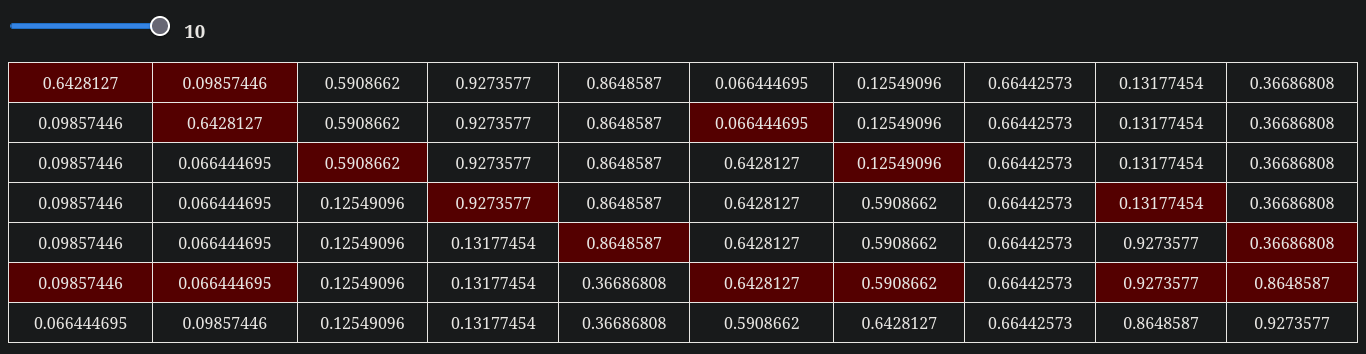
\includegraphics[scale=0.36]{1}
			\caption{Виконання програми}
		\end{figure}
		
		\section*{Висновок}
		під час виконання лабораторної роботи я вивчив алгоритм швидкого сортування. Здійснив програмну реалізацію алгоритму швидкого сортування. Дослідив швидкодію алгоритму швидкого сортування.
		
	\end{normalsize}
\end{document}
